% Current file is main.tex

%------------------------------------------------------------------------%
% Vorlage für Praxisarbeiten (o. Ä.) an der DHBW
%
% Autoren: Max Hüslbusch, Daniel Kerger
% Version: 1.0.0
% Datum:   09.05.2020
%------------------------------------------------------------------------%

% -- Präambel mit Angaben zum Dokument
\documentclass[
fontsize=12pt,          	 % Leitlinien sprechen von Schriftgröße 12.
paper=A4,
twoside=false,
listof=totoc,            		% Tabellen- und Abbildungsverzeichnis ins Inhaltsverzeichnis
index=totoc,				  %Stichwortverzeichnis wird in das Inhaltsverzeichniss aufgenommen
bibliography=totoc,		  % Literaturverzeichnis ins Inhaltsverzeichnis aufnehmen
titlepage,               % Titlepage-Umgebung anstatt \maketitle
headsepline,             % horizontale Linie unter Kolumnentitel
abstracton,              % Überschrift einschalten, Abstract muss in {abstract}-Umgebung stehen
ngerman
]{scrreprt}                  % Verwendung von KOMA-Report

\usepackage[onehalfspacing]{setspace}        % Zeilenabstand \singlespacing, \onehalfspaceing, \doublespacing
\usepackage{scrlayer-scrpage} 	   % Gestaltung von Fuß- und Kopfzeilen

\usepackage{titletoc}          			  % Anpassungen am Inhaltsverzeichnis
\contentsmargin{0.75cm}       		  % Abstand im Inhaltsverzeichnis zw. Punkt und Seitenzahl

% Paket für Quellen
\usepackage[
backend = biber,                % Verweis auf biber
language = auto,
style = numeric,                % Nummerierung der Quellen mit Zahlen
sorting = none,                 % none = Sortierung nach der Erscheinung im Dokument
sortcites = true,               % Sortiert die Quellen innerhalb eines cite-Befehls
block = space,                  % Extra Leerzeichen zwischen Blocks
hyperref = true,                % Links sind klickbar auch in der Quelle
%backref = true,                % Referenz, auf den Text an die zitierte Stelle
bibencoding = auto,
giveninits = true,              % Vornamen werden abgekürzt
doi=false,                      % DOI nicht anzeigen
isbn=false,                     % ISBN nicht anzeigen
alldates=short                  % Datum immer als DD.MM.YYYY anzeigen
]{biblatex}
\addbibresource{content/sources.bib}
\setcounter{biburlnumpenalty}{3000}     % Umbruchgrenze für Zahlen
\setcounter{biburlucpenalty}{6000}      % Umbruchgrenze für Großbuchstaben
\setcounter{biburllcpenalty}{9000}      % Umbruchgrenze für Kleinbuchstaben
\DeclareNameAlias{default}{family-given}  % Nachname vor dem Vornamen
\AtBeginBibliography{\renewcommand{\multinamedelim}{\addslash\space
	}\renewcommand{\finalnamedelim}{\multinamedelim}}  % Schrägstrich zwischen den Autorennamen
\DefineBibliographyStrings{german}{
	urlseen = {Einsichtnahme:},                      % Ändern des Titels von "besucht am"
}

% Unterstützung für Deutsch einbinden
\usepackage[ngerman]{babel}

% Pakete für die Darstellung von mathematischen Symbolen und Eingabemöglichkeit von Umlauten
\usepackage[T1]{fontenc}
\usepackage[utf8]{inputenc}
\usepackage[activate]{microtype}       % Trennung von Wörtern wird besser umgesetzt
\usepackage{lmodern}         % Nicht-gerasterte Schriftarten (bei MikTeX erforderlich)

\usepackage[babel,german=quotes]{csquotes}         % Deutsche Anführungszeichen + Zitate

% Pakete für Mathematik
\usepackage[sumlimits, intlimits]{amsmath}  % Bei Integralen und Summen werden die Zahlen oben drüber geschrieben 
\usepackage{amsmath}    % Erweiterung vom Mathe-Satz
\usepackage{amssymb}
\usepackage{amsfonts}
\usepackage{MnSymbol}   % Für Symbole, die in amssymb nicht enthalten sind.
\usepackage{array}
\usepackage{float}
\usepackage{mathtools}
\usepackage{mathrsfs}

% Pakete für Abkürzungen
\usepackage{acro}	%Abkürzungen werden nur gedruckt wenn sie gebraucht wurden
\acsetup{ list/display = used, pages/display = none }
%Currently no working solution due to package update
\DeclareAcronym{f}{
  short = \ensuremath{f} ,
  long  = Frequenz
}
\DeclareAcronym{A}{
  short = \ensuremath{A} ,
  long  = Fläche
}
\DeclareAcronym{C}{
  short = \ensuremath{C} ,
  long  = Kapazität
}
\DeclareAcronym{F}{
  short = \ensuremath{F} ,
  long  = Kraft
}

% \begin{acronym}[WYSISWG] % längstes Kürzel wird verw. für den Abstand zw. Kürzel u. Text
	
	% Alphabetisch selbst sortieren - nicht verwendete Kürzel rausnehmen!
	\DeclareAcronym{AIR}{
  		short = AIR,
  		long  = Adobe Integrated Runtime
	}
	% \acro{AJAX}{Asynchronous Javascript and XML}
	\DeclareAcronym{AJAX}{
  		short = AJAX,
  		long  = Asynchronous Javascript and XML
	}
	% \acro{ANSI}{American National Standards Institute}
	% \acro{API}{Application Programming Interface}
	\DeclareAcronym{API}{
		short = API,
		long  = Application Programming Interface
	}
	% \acro{AR}{Augmented Reality}
	% \acro{BAPI}{Business Application Programming Interface}
	% \acro{BIOS}{Basic Input Output System}
	% \acro{CDMA}{Code Division Multiple Access}
	% \acro{HTTPS}{Hypertext Transfer Protocol Secure}
	\DeclareAcronym{HTTPS}{
		short = HTTPS,
		long  = Hypertext Transfer Protocol Secure
	}
	% \acro{ISBN}{Internationale Standardbuchnummer}
	\DeclareAcronym{ISBN}{
		short = ISBN,
		long  = Internationale Standardbuchnummer
	}
	% \acrodefplural{ISBN}[ISBNs]{Internationale Standardbuchnummern}
	% \acro{OLAP}{Online Analytical Processing}
	% \acro{ORDBMS}{Object-Relational DataBase Management System}
	% \acro{SDK}{Software Development Kit}
	% \acro{SEO}{Search Engine Optimization}
	% \acro{SSH}{Secure Shell}
	% \acro{UEFI}{Unified Extensible Firmware Interface}
	% \acro{USB}{Universal Serial Bus}
	% \acro{VLAN}{Virtual Local Area Network}
	% \acro{WYSISWG}{What You See Is What You Get}
	% \acro{XSL}{Extensible Stylesheet Language}
	
% \end{acronym}

% Pakete für Tabellen
\usepackage{booktabs}  % Für schönere Tabellen. Enthält neue Befehle wie \midrule
\usepackage{multirow}  % Mehrzeilige Tabellen
\usepackage{siunitx}   % Für SI Einheiten und das Ausrichten Nachkommastellen
\sisetup{locale=DE, range-phrase={~bis~}, output-decimal-marker={,}} % Damit ein Komma und kein Punkt verwendet wird.
\usepackage{xfrac} % Für siunitx Option "fraction-function=\sfrac"
\setlength{\tabcolsep}{10pt}					% Abstand des Inhalts zur Linie
\renewcommand{\arraystretch}{1.25}		%Abstand der Zeilen wird erhöht 1.0 ist default

% Pakete für Bilder
\usepackage{wrapfig}
\usepackage{graphicx}
\usepackage{caption}

% Pakete für Definitionsboxen
\usepackage{amsthm}                     % Liefert die Grundlagen für Theoreme
\usepackage[framemethod=tikz]{mdframed} % Boxen für die Umrandung
% ---- Definition für Highlight Boxen

% ---- Grundsätzliche Definition zum Style
\newtheoremstyle{defi}
  {\topsep}         % Abstand oben
  {\topsep}         % Abstand unten
  {\normalfont}     % Schrift des Bodys
  {0pt}             % Einschub der ersten Zeile
  {\bfseries}       % Darstellung von der Schrift in der Überschrift
  {:}               % Trennzeichen zwischen Überschrift und Body
  {.5em}            % Abstand nach dem Trennzeichen zum Body Text
  {\thmname{#3}}    % Name in eckigen Klammern
\theoremstyle{defi}

% ------ Definition zum Strich vor eines Texts
\newmdtheoremenv[
  hidealllines = true,       % Rahmen komplett ausblenden
  leftline = true,           % Linie links einschalten
  innertopmargin = 0pt,      % Abstand oben
  innerbottommargin = 4pt,   % Abstand unten
  innerrightmargin = 0pt,    % Abstand rechts
  linewidth = 3pt,           % Linienbreite
  linecolor = gray!40,       % Linienfarbe
]{defStrich}{Definition}     % Name der des formats "defStrich"

% ------ Definition zum Eck-Kasten um einen Text
\newmdtheoremenv[
  hidealllines = true,
  innertopmargin = 6pt,
  linecolor = gray!40,
  singleextra={              % Eck-Markierungen für die Definition
    \draw[line width=3pt,gray!50,line cap=rect] (O|-P) -- +(1cm,0pt);
    \draw[line width=3pt,gray!50,line cap=rect] (O|-P) -- +(0pt,-1cm);
    \draw[line width=3pt,gray!50,line cap=rect] (O-|P) -- +(-1cm,0pt);
    \draw[line width=3pt,gray!50,line cap=rect] (O-|P) -- +(0pt,1cm);
  }
]{defEckKasten}{Definition}  % Name der des formats "defEckKasten"  % Weitere Details sind ausgelagert

% Pakete für Aufzählungen
\usepackage{enumitem}

% Pakete für Referenzen
\usepackage{varioref}
\usepackage[                        % Klickbare Links (enth. auch "nameref", "url" Package)
hidelinks,                    			 % Blende die "URL Boxen" aus.
breaklinks=true              	    % Breche zu lange URLs am Zeilenende um
]{hyperref}

\hypersetup{%
	linktocpage=true, 		% Nicht der Text sondern die Seitenzahlen in Verzeichnissen klickbar
	bookmarksnumbered=true 	% Überschriftsnummerierung im PDF Inhalt anzeigen.
}
\usepackage[noabbrev]{cleveref}   %Kein erkennen von Abkürzungen 

% Quellcodevorlage
\usepackage{scrhack}                    % Hack zur Verw. von listings in KOMA-Script
\usepackage{listings}                   % Darstellung von Quellcode
\usepackage{xcolor}                     % Einfache Verwendung von Farben
% -- Eigene Farben für den Quellcode
\definecolor{JavaLila}{rgb}{0.4,0.1,0.4}
\definecolor{JavaGruen}{rgb}{0.3,0.5,0.4}
\definecolor{JavaBlau}{rgb}{0.0,0.0,1.0}
\definecolor{ABAPKeywordsBlue}{HTML}{6000ff}
\definecolor{ABAPCommentGrey}{HTML}{808080}
\definecolor{ABAPStringGreen}{HTML}{4da619}
\definecolor{PyKeywordsBlue}{HTML}{0000AC}
\definecolor{PyCommentGrey}{HTML}{808080}
\definecolor{PyStringGreen}{HTML}{008080}
% -- Farben für ABAP CDS
\definecolor{CDSString}{HTML}{FF8C00}
\definecolor{CDSKeywords}{HTML}{6000ff}
\definecolor{CDSAnnotation}{HTML}{00BFFF}
\definecolor{CDSComment}{HTML}{808080}
\definecolor{CDSFunc}{HTML}{FF0000}
% -- Farben für C++
\definecolor{C++Lila}{HTML}{A640FF}
\definecolor{C++Orange}{HTML}{D69D85}
\definecolor{C++Blau}{HTML}{569CD6}
\definecolor{C++DunkelBlau}{HTML}{0E4583}
\definecolor{C++Mint}{HTML}{B8D7A3}
\definecolor{C++Creme}{HTML}{DCDCAA}
\definecolor{C++Gruen}{HTML}{57A64A}
\definecolor{C++Tuerkis}{HTML}{4EC9B0}

% -- Default Listing-Styles

\lstset{
	% Das Paket "listings" kann kein UTF-8. Deswegen werden hier 
	% die häufigsten Zeichen definiert (ä,ö,ü,...)
	literate=%
		{á}{{\'a}}1 {é}{{\'e}}1 {í}{{\'i}}1 {ó}{{\'o}}1 {ú}{{\'u}}1
		{Á}{{\'A}}1 {É}{{\'E}}1 {Í}{{\'I}}1 {Ó}{{\'O}}1 {Ú}{{\'U}}1
		{à}{{\`a}}1 {è}{{\`e}}1 {ì}{{\`i}}1 {ò}{{\`o}}1 {ù}{{\`u}}1
		{À}{{\`A}}1 {È}{{\'E}}1 {Ì}{{\`I}}1 {Ò}{{\`O}}1 {Ù}{{\`U}}1
		{ä}{{\"a}}1 {ë}{{\"e}}1 {ï}{{\"i}}1 {ö}{{\"o}}1 {ü}{{\"u}}1
		{Ä}{{\"A}}1 {Ë}{{\"E}}1 {Ï}{{\"I}}1 {Ö}{{\"O}}1 {Ü}{{\"U}}1
		{â}{{\^a}}1 {ê}{{\^e}}1 {î}{{\^i}}1 {ô}{{\^o}}1 {û}{{\^u}}1
		{Â}{{\^A}}1 {Ê}{{\^E}}1 {Î}{{\^I}}1 {Ô}{{\^O}}1 {Û}{{\^U}}1
		{œ}{{\oe}}1 {Œ}{{\OE}}1 {æ}{{\ae}}1 {Æ}{{\AE}}1 {ß}{{\ss}}1
		{ű}{{\H{u}}}1 {Ű}{{\H{U}}}1 {ő}{{\H{o}}}1 {Ő}{{\H{O}}}1
		{ç}{{\c c}}1 {Ç}{{\c C}}1 {ø}{{\o}}1 {å}{{\r a}}1 {Å}{{\r A}}1
		{€}{{\euro}}1 {£}{{\pounds}}1 {«}{{\guillemotleft}}1
		{»}{{\guillemotright}}1 {ñ}{{\~n}}1 {Ñ}{{\~N}}1 {¿}{{?`}}1,
	breaklines=true,        % Breche lange Zeilen um 
	breakatwhitespace=true, % Wenn möglich, bei Leerzeichen umbrechen
	% Symbol für Zeilenumbruch einfügen
	prebreak=\raisebox{0ex}[0ex][0ex]{\ensuremath{\rhookswarrow}},
	postbreak=\raisebox{0ex}[0ex][0ex]{\ensuremath{\rcurvearrowse\space}},
	tabsize=4,                                 % Setze die Breite eines Tabs
	basicstyle=\ttfamily\small,                % Grundsätzlicher Schriftstyle
	columns=fixed,                             % Besseres Schriftbild
	numbers=left,                              % Nummerierung der Zeilen
	%frame=single,                             % Umrandung des Codes
	showstringspaces=false,                    % Keine Leerzeichen hervorheben
	keywordstyle=\color{blue},
	ndkeywordstyle=\bfseries\color{darkgray},
	identifierstyle=\color{black},
	commentstyle=\itshape\color{JavaGruen},   % Kommentare in eigener Farbe
	stringstyle=\color{JavaBlau},             % Strings in eigener Farbe,
	captionpos=b                             % Bild*unter*schrift
}

% ---- Eigener JAVA-Style für den Quellcode
\renewcommand{\ttdefault}{pcr}               % Schriftart, welche auch fett beinhaltet
\lstdefinestyle{EigenerJavaStyle}{
	language=Java,                             % Syntax Highlighting für Java
	%frame=single,                             % Umrandung des Codes
	keywordstyle=\bfseries\color{JavaLila},    % Keywords in eigener Farbe und fett
	commentstyle=\itshape\color{JavaGruen},    % Kommentare in eigener Farbe und italic
	stringstyle=\color{JavaBlau}               % Strings in eigener Farbe
}

% ---- Eigener ABAP-Style für den Quellcode
\renewcommand{\ttdefault}{pcr}
\lstdefinestyle{EigenerABAPStyle}{
	language=[R/3 6.10]ABAP,
	morestring=[b]\|,                          % Für Pipe-Strings
	morestring=[b]\`,                          % für Backtick-Strings
	keywordstyle=\bfseries\color{ABAPKeywordsBlue},
	commentstyle=\itshape\color{ABAPCommentGrey},
	stringstyle=\color{ABAPStringGreen},
	tabsize=2,
	morekeywords={
		types,
		@data,
		as,
		lower,
		start,
		selection,
		order,
		by,
		inner,
		join,
		key,
		end,
		cast
	}
}

% ---- Eigener Python-Style für den Quellcode
\renewcommand{\ttdefault}{pcr}
\lstdefinestyle{EigenerPythonStyle}{
	language=Python,
	columns=flexible,
	keywordstyle=\bfseries\color{PyKeywordsBlue},
	commentstyle=\itshape\color{PyCommentGrey},
	stringstyle=\color{PyStringGreen}
}

%----- ABAP-CDS-View language
\lstdefinelanguage{ABAPCDS}{
	sensitive=false,
	%Keywords
	morekeywords={define,
		view,
		as,
		select,
		from,
		inner,
		join,
		on,
		key,
		case,
		when,
		then,
		else,
		end,
		true,
		false,
		cast,
		where,
		and,
		distinct,
		group,
		by,
		having,
		min,
		sum,
		max,
		count,
		avg
	},
	%Methoden
	morekeywords=[2]{
		div,
		currency\_conversion,
		dats\_days\_between,
		concat\_with\_space,
		dats\_add_days,
		dats\_is\_valid,
		dats\_add\_months,
		unit\_conversion,
		division,
		mod,
		abs,
		floor,
		ceil,
		round,
		concat,
		replace,
		substring,
		left,
		right,
		length
	},
	morecomment=[s][\color{CDSAnnotation}]{@}{:},
	morecomment=[l][\itshape\color{CDSComment}]{//},
	morecomment=[s][\itshape\color{CDSComment}]{/*}{*/},
	morestring=[b][\color{CDSString}]',
	keywordstyle=\bfseries\color{CDSKeywords},
	keywordstyle=[2]\color{CDSFunc}
}


% ---- Eigener XSD-Style für den Quellcode
\renewcommand{\ttdefault}{pcr}
\lstdefinestyle{EigenerXSDStyle}{
	language=XML,                     
	stringstyle=\color{JavaGruen},
	morekeywords={
		encoding,
		xs:schema,
		xs:element,
		xs:complexType,
		xs:sequence,
		xs:attribute,
		xs:simpleContent,
		xs:extension base, 
		encoding,
		schema,
		element,
		complexType,
		sequence,
		attribute,
		simpleContent,
		extension base
	}
}

% ---- Eigener C++-Style für den Quellcode
\renewcommand{\ttdefault}{pcr}               % Schriftart, welche auch fett beinhaltet
\lstdefinestyle{EigenerC++Style}{
	language=C++,			% Standardsprache des Quellcodes
    columns=flexible,
	morekeywords={nullptr},
	% Enumerators (Mint)
	morekeywords=[2]{},
    % Methoden (Cremefarben)
	morekeywords=[3]{},
	% Extra Keywords (Lila)
	morekeywords=[4]{},
	% Noch mehr Keywords (Gruen)
	morekeywords=[5]{},
    keywordstyle=\bfseries\color{C++DunkelBlau},
    keywordstyle=[2]\color{C++Mint},
    keywordstyle=[3]\color{C++Creme},
    keywordstyle=[4]\color{C++Lila},
    keywordstyle=[5]\color{C++Tuerkis},
	commentstyle=\itshape\color{C++Gruen},
	stringstyle=\color{C++Orange}
}  % Weitere Details sind ausgelagert
\usepackage{algorithm}                  % Für Algorithmen-Umgebung (ähnlich wie lstlistings Umgebung)
\usepackage{algpseudocode}              % Für Pseudocode. Füge "[noend]" hinzu, wenn du kein "endif",
% etc. haben willst.
\makeatletter                           % Sorgt dafür, dass man @ in Namen verwenden kann.
% Ansonsten gibt es in der nächsten Zeile einen Compilefehler.
\renewcommand{\ALG@name}{Algorithmus}   % Umbenennen von "Algorithm" im Header der Listings.
\makeatother                            % Zeichen wieder zurücksetzen
\renewcommand{\lstlistingname}{Listing} % Erlaubt das Umbenennen von "Listing" in anderen Titel.

% Anhänge werden sortiert
\usepackage[titletoc]{appendix} %Fügt "Anhang" in TOC ein. 

% Paket für ein Stichwortverzeichnis
\usepackage{makeidx}
\makeindex

% Nur ein latex-Durchlauf für die Aktualisierung von Verzeichnissen nötig
\usepackage{bookmark} 

% Zeilenumbruch, Seitenränder und mehr
\usepackage[
%showframe,                % Ränder anzeigen lassen
left=2.7cm, right=2.5cm,
top=2.5cm,  bottom=2.5cm,
includeheadfoot
]{geometry}                 

% Schriftart wird geändert
\usepackage{lmodern}
\renewcommand*\familydefault{\sfdefault} 				%Serifenlose Schrift 

%Unterüberschriften 
\usepackage[list=true]{subcaption} %Unterbilder werden im Abbildungsverzeichniss dargestellt 


% Bildunterschriften werden etwas kleiner dargestellt
\addtokomafont{caption}{\small}

\addto\extrasngerman{%
	\def\equationautorefname~#1\null{Gleichung~(#1)\null}
	\def\lstnumberautorefname{Zeile}
	\def\lstlistingautorefname{Listing}
	\def\algorithmautorefname{Algorithmus}
	% Damit einheitlich "Abschnitt 1.2[.3]" verwendet wird und nicht "Unterabschnitt 1.2.3"
	% \def\subsectionautorefname{Abschnitt}
}

% ---- Abstand verkleinern von der Überschrift 
\renewcommand*{\chapterheadstartvskip}{\vspace*{.5\baselineskip}}

% Einzelne Wörter
\widowpenalty10000
\clubpenalty10000

% Paket für Blindtext
\usepackage{lipsum}

% Layout für die Absätze
\setlength{\parindent} {0.0em}
\setlength{\parskip} {1.5ex plus0.5ex minus0.5ex}   % Setzt den Abstand zwischen 2 Absätzen 

% Mehrere Spalten auf einer Seite 
\usepackage{multicol}

% Rotieren einer einzelnen PDF-Seite in der landscape Umgebung
\usepackage{pdflscape}

% Aufsetzen von Variablen
\usepackage{ifthen}
\newboolean{durchgehendeFussnoten}
\newboolean{sperrvermerkLangeVersion}
\newboolean{abgabeVersion}

% Ermöglichen von Umbrüchen in Tabellen
\usepackage{makecell}

% Glossar
\usepackage[nonumberlist,toc]{glossaries}

% Standardpfad für Bilder wird angepasst, sodass nur noch der Dateiname des Bildes angegeben werden muss.
\graphicspath{{images/}}

\acsetup{ list/display = all , pages/display = all}

\usepackage{longtable,siunitx}


% -- Änderungen an Schreibweisen und Silbentrennungen
% ---- Hilfreiches
\newcommand{\zB}{z.\,B. }   % "z.B." mit kleinem Leeraum dazwischen (ohne wäre nicht korrekt)
\newcommand{\dash}{d.\,h. }

% ---- Silbentrennung (falls LaTeX defaults falsch / nicht gewünscht sind)
\hyphenation{HANA}         % anstatt HA-NA
\hyphenation{Graph-Script} % anstatt GraphS-cript

% -- Allgemeine Informationen zur Arbeit
\newcommand{\titel}{Beispieltitel, welcher am Besten über zwei Zeilen verläuft}
\newcommand{\titelheader}{Titel welcher im Header auftaucht}
\newcommand{\arbeit}{Projektarbeit 1 (T1\_1000)}

% -- Persönliche Angaben und DHBW
\newcommand{\vorname}{Max}
\newcommand{\nachname}{Mustermann}
\newcommand{\matrikelnr}{1234567}
\newcommand{\kurs}{AB12CDE}
\newcommand{\studiengang}{Musterstudiengang}
\newcommand{\studienjahr}{2019}
\newcommand{\abschluss}{Bachelor of Muster}
\newcommand{\betreuerDhbw}{DH-Vorname DH-Nachname}

% -- Angaben zum Zeitraum
\newcommand{\bearbeitungsmonat}{Februar 2020}
\newcommand{\abgabeOrt}{Musterort}
\newcommand{\abgabeDatum}{08. September 2020}
\newcommand{\bearbeitungszeitraum}{24.03.2020 - 08.09.2020}

% -- Angaben zu der Ausbildungsfirma
\newcommand{\firmaName}{Musterfirma}
\newcommand{\firmaStrasse}{Musterstraße 4711}
\newcommand{\firmaPlz}{00000 Musterort, Deutschland}
\newcommand{\betreuerFirma}{B-Vorname B-Nachname}

% -- Zusätzliche Optionen 
\setboolean{durchgehendeFussnoten}{true}		% Die Fußnoten werden nicht nach jedem Kapitel neu gezählt
\setboolean{sperrvermerkLangeVersion}{true}		% Es soll eine lange Version des Sperrvermerks eingebunden werden
\setboolean{abgabeVersion}{false} 				% ToDo-Notes und andere Dokumente werden ausgeblendet. Dies ist die Abgabe Version.
% Current file is content/00_LaTeX/variables/runVariables

\ifthenelse{\boolean{durchgehendeFussnoten}}
{
	\usepackage{chngcntr}
	\counterwithout{footnote}{chapter}
}
{}
\ifthenelse{\boolean{abgabeVersion}}
{
	% Pakete Für Todo Notes
	\usepackage[disable]{todonotes}
	\setlength {\marginparwidth }{2cm}      % Abstand für Todo Notizen
}
{
	% Pakete Für Todo Notes
	\usepackage{todonotes}
	\setlength {\marginparwidth }{2cm}      % Abstand für Todo Notizen
}

\ifthenelse{\not\boolean{abgabeVersion}\and\boolean{anleitungDrucken}}							
{
	\addbibresource{content/00_LaTeX/exampleProject/exampleSources.bib}
}
{}	% Einstellungen der Variablen werden ausgeführt

% -- Glossar
\makeglossaries									% Glossarfunktionen werden initialisiert
% Current file is content/07_appendix/glossary.tex

% Anleitung für das Glossar:
% 1. Normaler LaTeX Kompiliervorgang und nicht die Auxiliary Files löschen
% 2. In der Konsole den Befehl makeglossaries main ausführen
% 3. Abschließender LaTex Kompiliervorgang

% Glossareintraege --> referenz, name, beschreibung
% Aufruf mit \gls{...}
 
\newglossaryentry{Glossareintrag}
{   
    name={Glossareintrag},
    plural={Glossareinträge},
    description={Ein Glossar beschreibt verschiedenste Dinge in kurzen Worten}
}			% Glossareinträge werden ausgelesen

% -- Kopf- und Fußzeilen
% Current file is content/00_LaTeX/miscellanious/headerAndFooter.tex

% -- Metainformation für das PDF Dokument
% Hier werden die Metainformationen für das generierte PDF Dokument hinterlegt. Eingesehen werden können diese Informationen in Acrobat unter Datei -> Eigenschaften.
\hypersetup{
    pdftitle    = {\titel},
    pdfsubject  = {\arbeit},
    pdfauthor   = {\nachname, \vorname},
    pdfcreator  = {LaTeX}
}

% -- Definition der Kopf- und Fußzeilen
\clearscrheadfoot                               % Löschen von LaTeX Standard
\automark[section]{chapter}                     % Füllen von section und chapter
\renewcommand*{\chaptermarkformat}{}            % Entfernt die Kapitelnummer
\renewcommand*{\sectionmarkformat}{}            % Entfernt die Sectionnummer
% Angaben [für "plain"]{für "scrheadings"}
\ihead[]{\titelheader}                          % Kopfzeile links
\chead[]{}                                      % Kopfzeile mitte
\ohead[]{\rightmark}                            % Kopfzeile rechts
\ifoot[]{}                                      % Fußzeile links
\cfoot*{\sffamily\pagemark}                     % Fußzeile mitte
\ofoot[]{}                                      % Fußzeile rechts
\KOMAoptions{
   headsepline = 0.2pt,                         % Liniendicke Kopfzeile
   footsepline = false                          % Liniendicke Fußzeile
}	% Layout der Kopf- und Fußzeilen werden eingelesen

\begin{document}
	\setlength{\parindent}{0pt}              	% Keine Paragraphen Einrückung.
	\setcounter{secnumdepth}{2}             	% Nummerierungstiefe fürs Inhaltsverzeichnis
	\setcounter{tocdepth}{1}             	    % Tiefe des Inhaltsverzeichnisses. Ggf. so anpassen, dass das Verzeichnis auf eine Seite passt.
	\sffamily                                	% Serifenlose Schrift verwenden.
	
	% -- Einbinden des Deckblatts
	\singlespacing								% Einfacher Zeilenabstand
    \thispagestyle{empty}
\begin{titlepage}
	\enlargethispage{4cm}
	\begin{figure}
		% \vspace*{-5mm} 
		\begin{minipage}{0.49\textwidth}
			\flushleft
			\missingfigure[figheight=2.5cm, figcolor=white]{Insert company logo here} 
			%\includegraphics[height=2.5cm]{images/logos/...} 
		\end{minipage}
		\hfill
		\begin{minipage}{0.49\textwidth}
			\flushright
			
\includegraphics[height=2.5cm]{images/logos/dhbw.png} 
		\end{minipage}
	\end{figure} 
	\vspace*{0.1cm}
	\begin{center}
		\huge{\textbf{\titel}}\\[1.5cm]
		\Large{\textbf{\arbeit}}\\[0.5cm]
		\normalsize{im Rahmen der Prüfung zum\\[1ex] \textbf{Bachelor of Muster}}\\[0.5cm]
		\Large{des Studienganges \studiengang}\\[1ex]
		\normalsize{an der Dualen Hochschule Baden-Württemberg Stuttgart}\\[1cm]
		\normalsize{von}\\[1ex] \Large{\textbf{\autor}} \\[1cm]
		\normalsize{\bearbeitungsmonat}\\[2.25cm]
		\begin{spacing}{0.8}
			\begin{tabular}{ll}
				\textbf{Abgabedatum}				\hspace{4.5cm}					& \abgabeDatum\\[0.2cm]
				\textbf{Bearbeitungszeitraum}       				&  \bearbeitungszeitraum\\[0.2cm]
				\textbf{Matrikelnummer, Kurs} 					   	&  \matrikelnr, \kurs\\[0.2cm]
				\textbf{Ausbildungsfirma}              					 &  \firmaName\\
																						& \firmaStrasse \\
																				    	& \firmaPlz\\[0.2cm]
				\textbf{Betreuer der Ausbildungsfirma}          &  \betreuerFirma\\[0.2cm]
				\textbf{Gutachter der Dualen Hochschule}    &  \betreuerDhbw\\[0.2cm]
			\end{tabular} 
		\end{spacing}
	\end{center}
\end{titlepage}
	% Titelseite wird eingebunden
    \newcounter{savepage}						% Zähler für die römischen Zahlen wird erstellt.
    \pagenumbering{Roman} 						% Seitenzahlen werden durch römische Buchstaben gekennzeichnet
    \onehalfspacing								% Eineinhalbfacher Zeilenabstand
    
    % -- Einbinden der Erklärung
    % Current file is content/02_declaration/declaration.tex
% LTex: language=en-EN
\ifthenelse{\boolean{englischeVersion}}
{
	\chapter*{Declaration}
	Hereby I solemnly declare that this {\arbeit}, titled:
	\begin{quote}
		\textit{\titel}
	\end{quote}
	is entirely the product of my own scholarly work and I have indicated the thoughts adopted directly or indirectly from other sources at the appropriate places within the document. In addition I assure, that the printed version is equivalent to the submitted electronic one.
	\vspace{1cm}

	\abgabeOrt, the \printdate{\abgabeDatum} \\[0.5cm]
	{\makebox[6cm]{\hrulefill}}\\ 
	\nachname , \vorname
}
% LTex: language=de-DE
{
	\chapter*{Erklärung}
		Ich versichere hiermit, dass ich meine \arbeit{} mit dem Thema:
		\begin{quote}
			\textit{\titel}
		\end{quote}
		selbstständig verfasst und keine anderen als die angegebenen Quellen und Hilfsmittel benutzt habe. Ich versichere zudem, dass die eingereichte elektronische Fassung mit der gedruckten Fassung übereinstimmt. 
		\vspace{1cm}
		
		\abgabeOrt, den \printdate{\abgabeDatum} \\[0.5cm]
		{\makebox[6cm]{\hrulefill}}\\ 
		\nachname , \vorname
}

    
    % -- Einbinden des Sperrvermerks
    % Current file is content/03_confidentiallyStatement/confidentiallyStatement.tex


\ifthenelse{\boolean{englischeVersion}}
{
	\chapter*{Confidentially Statement}
	The {\arbeit} on hand:
	\begin{quote}
		\textit{\titel}
	\end{quote}
 	contains internal resp.\ confidential data of {\firmaName}. It is intended solely for inspection by the assigned examiner, the head of the {\studiengang} department and, if necessary, the Audit Committee of the Baden-Wuerttemberg Cooperative State University \abgabeOrt. It is strictly forbidden
  	\begin{itemize}
		\item to distribute the content of this paper (including data, figures, tables, charts etc.) as a whole or in extracts,
		\item to make copies or transcripts of this paper or of parts of it,
		\item to display this paper or make it available in digital, electronic or virtual form.
  	\end{itemize}
	Exceptional cases may be considered through permission granted in written form by the author and {\firmaName}.
}
{
	\chapter*{Sperrvermerk}
	\ifthenelse{\boolean{sperrvermerkLangeVersion}}
	{
		Die vorliegende {\arbeit} mit dem Titel: 
		\begin{quote}
			\textit{\titel}
		\end{quote}
		enthält unternehmensinterne bzw. vertrauliche Informationen der {\firmaName}, ist deshalb mit einem Sperrvermerk versehen und wird ausschließlich zu Prüfungszwecken am Studiengang {\studiengang} der Dualen Hochschule Baden-Württemberg {\abgabeOrt} vorgelegt. Sie ist ausschließlich zur Einsicht durch den zugeteilten Gutachter, die Leitung des Studiengangs und ggf. den Prüfungsausschuss des Studiengangs bestimmt.  Es ist untersagt,
		\begin{itemize}
			\item den Inhalt dieser Arbeit (einschließlich Daten, Abbildungen, Tabellen, Zeichnungen usw.) als Ganzes oder auszugsweise weiterzugeben,
			\item Kopien oder Abschriften dieser Arbeit (einschließlich Daten, Abbildungen, Tabellen, Zeichnungen usw.) als Ganzes oder in Auszügen anzufertigen,
			\item diese Arbeit zu veröffentlichen bzw. digital, elektronisch oder virtuell zur Verfügung zu stellen. 
		\end{itemize}
		Jede anderweitige Einsichtnahme und Veröffentlichung – auch von Teilen der Arbeit – bedarf der vorherigen Zustimmung durch den Verfasser und {\firmaName}.
	}
	{
		Der Inhalt dieser Arbeit darf weder als Ganzes noch in Auszügen Personen außerhalb des Prüfungsprozesses und des Evaluationsverfahrens zugänglich gemacht werden, sofern keine anderslautende Genehmigung der Ausbildungsstätte vorliegt.
	}
}
    
    % -- Einbinden des Abstracts
    % Current file is content/04_abstract/abstract-de.tex

\renewcommand{\abstractname}{Abstract} % Veränderter Name für das Abstract
\begin{abstract}
\begin{addmargin}[1.5cm]{1.5cm}        % Erhöhte Ränder, für Abstract Look
\thispagestyle{plain}                  % Seitenzahl auf der Abstract Seite

\begin{center}
\small\textit{- Deutsch -}             % Angabe der Sprache für das Abstract
\end{center}

\vspace{0.25cm}

Dies ist der Beginn des Abstracts. Für die finale Bachelorarbeit musst du ein Abstract in deinem Dokument mit einbauen. So, schreibe es am besten jetzt in Deutsch und Englisch. Das Abstract ist eine kurze Zusammenfassung mit ca. 200 bis 250 Wörtern.

\vspace{0.25cm}

Versuche in das Abstract folgende Punkte aufzunehmen: Fragestellung der Arbeit, methodische Vorgehensweise oder die Hauptergebnisse deiner Arbeit.


\end{addmargin}
\end{abstract}
    % Current file is content/04_abstract/abstract-en.tex

\renewcommand{\abstractname}{Abstract} % Veränderter Name für das Abstract
\begin{abstract}
\begin{addmargin}[1.5cm]{1.5cm}        % Erhöhte Ränder, für Abstract Look
\thispagestyle{plain}                  % Seitenzahl auf der Abstract Seite

\begin{center}
\small\textit{- English -}             % Angabe der Sprache für das Abstract
\end{center}

\vspace{0.25cm}

This is the starting point of the Abstract. For the final bachelor thesis, there must be an abstract included in your document. So, start now writing it in German and English. The abstract is a short summary with around 200 to 250 words.

\vspace{0.25cm}

Try to include in this abstract the main question of your work, the methods you used or the main results of your work.


\end{addmargin}
\end{abstract}
    
    % -- Inhaltsverzeichnis
    \singlespacing													% Einfacher Zeilenabstand
    \tableofcontents												% Inhaltsverzeichnis wird erstellt

	% -- Verzeichnisse
	\renewcommand*{\chapterpagestyle}{plain}						% Kapitel-Style wird auf plain gestellt 
	\pagestyle{plain}												% Seiten-Style wird auf plain gestellt
	\printacronyms[template=physics, include=physics, name=Formelverzeichnis]		%TBR
	\printacronyms[template=physics, exclude=physics, name=Abkürzungsverzeichnis]	%TBR

	\listoffigures                         							% Erzeugen des Abbildungsverzeichnisses 
	\listoftables                          							% Erzeugen des Tabellenverzeichnisses
    \renewcommand{\lstlistlistingname}{Quellcodeverzeichnis}		% Umbenennung des Quellcodeverzeichisses
    \lstlistoflistings                     							% Erzeugen des Listenverzeichnisses
    \setcounter{savepage}{\value{page}}								% Römische Seitenzahl wird für später gespeichert

	% -- Liste der zu erledigenden Punkte. Wichtig: Diese Liste muss vor der endgültigen Abgabe auskommentiert werden!
	\listoftodos
    
    % -- Einbinden von den verschiedenen Kapiteln
    \cleardoublepage												% Beendet eine Seite
    \pagenumbering{arabic}                							% Arabische Seitenzahlen für den Hauptteil
    \setlength{\parskip}{0.5\baselineskip}  						% Abstand zwischen Absätzen wird geändert
    \rmfamily														% Schriftfamilie wird festgelegt
    \renewcommand*{\chapterpagestyle}{scrheadings}					% Kapitel-Style wird auf scrheadings gestellt 
    \pagestyle{scrheadings}											% Seiten-Style wird auf scrheadings gestellt
    \onehalfspacing													% Eineinhalbfacher Zeilenabstand
	\sffamily                               					 	% Serifenlose Schrift verwenden. 
	   
	\ifthenelse{\boolean{abgabeVersion}}							% Beispielkapitel werden eingebunden
	{}
	{
		\chapter{Einleitung}

\section*{Information bezüglich des Inhaltsverzeichnisses}
Nachtrag zum Inhaltsverzeichnis: Dieses sollte wenn möglich nur eine Seite lang sein. Unterpunkte können dabei auch ausgelassen werden. Dies kann ganz einfach durchgeführt werden indem die section mit einen Stern geschrieben wird, wie bei der Sektion hier.

Des Weiteren solltest du beachten, dass du keine Unterpunkte alleine aufmachen darfst. Laut den DHBW Leitlinien sollte, wenn es einen Punkt 1.1 gibt, auch ein Punkt 1.2 existieren. Weitere Details dazu in den Leitlinien - zur Info: diese Vorlage hält sich aktuell nicht an diese Regelung, sie ist schließlich nur ein Template.

\section{Grobe Struktur der Arbeit}
Alle Details zur Struktur findest du in den Leitlinien ab Seite 21. Nachfolgend ist nur die verkürze Version mit allen wichtigen Punkten angegeben.

\subsection{Einleitung - was gibt es zu beachten?}
Die Einleitung sollte folgende Punkte beinhalten:
\begin{itemize}
\item \textbf{Gegenstand und Ziele der Arbeit \& Aufgabenbeschreibung, Einführung in Thema, Stand der Technik \& Forschung, Motivation der Aufgabenstellung \& Vorausblick}
\item Ausgangspunkt der Arbeit umreisen
\item Hinführung zur Problemstellung + Interesse des Lesers wecken
\item Allgemeine Einleitung ins Thema (keine Unternehmens-, Produktbeschreibungen oder Organigramme!)
\item Fragestellung präsentieren, Motivation erläutern
\item Randbedingungen und Betrachtungsgrenzen aufzeigen
\item Stand der Technik und aktuelle Lösungsfindung beschreiben, Vor- und Nachteile bisheriger Lösung anhand von Literatur darlegen
\end{itemize}

\subsection{Hauptteil - zeige was du kannst!}
Folgende Punkte kannst du in deinen Hauptteil einarbeiten:
\begin{itemize}
\item \textbf{Anforderungsdefinition, Anforderungsanalyse, Lösungsgenerierung, Lösungsbewertung, Umsetzung) in sinnvollen Gliederungspunkten}
\item Gewähltes Verfahren oder bestimmter Lösungsweg muss begründet werden
\item Bei Versuchen (nicht alle müssen genannt werden) müssen Voraussetzungen, Vernachlässigungen sowie Anordnung, Leistungsfähigkeit und Messgenauigkeit der einzelnen Versuchsanordnung angeben werden
\item Ergebnisse der Arbeit ausführlich diskutieren, Vergleiche mit Anschauungen und Erfahrungen vergleichen
\item Ziel der Arbeit: Eindeutige Folgerungen und Richtlinien für die Praxis
\end{itemize}

\subsection{Schluss - das Ziel ist nahe...}
Nachfolgende Aspekte können in den Schluss eingearbeitet werden:
\begin{itemize}
\item \textbf{Zusammenfassung und Ausblick}
\item Aufgabenstellung, Vorgehensweise, sowie wesentliche Ergebnisse kurz/präzise darstellen
\item Zusammenfassung eigenständig verständlich
\item Länge ca. 1-1,5 Seiten (Problem, Ziele, Vorgehensweise, Ergebnisse und Ausblick)
\end{itemize}

\subsection{Sonstige Tipps}
Es ist hilfreich, sich Notizen in das Dokument zu schreiben.
\LaTeX Kommentare haben jedoch den Nachteil, dass sie in der PDF nicht erscheinen.
Einfacher Text wird auch leicht überlesen.
Deshalb wird in dieser Vorlage das Package ToDoNotes eingebunden, welches Notizen in dem Dokument sichtbar macht.\todo{So wie hier}
Auf der rechten Seite siehst du ein Beispiel.

Ein Glossareintrag kann mit dem Befehl \texttt{gls} erstellt werden. Ein Beispielglossareintrag \gls{Glossareintrag}.

		% LTeX: enabled=false
\chapter{Abbildungen}
Alle Abbildungen und Tabellen sind laut Richtlinien fortlaufend mit Nummern zu versehen. Diese Aufgabe übernimmt \LaTeX{} für dich. Jedoch solltest du den Text unter dem Bild (Legende) auf das jeweilige Bild anpassen. Hast du das Bild irgendwo entnommen, dann muss der Quellenverweis auch direkt in der Legende mit eingebaut sein.

Im Text selbst solltest du auf die Abbildung verweisen. Neben dem reinen verweisen, solltest du dich auch damit auseinandersetzen. Beschreibe die Grafik, hebe die Relevanz einzelner Teile hervor oder nenne andere wichtige Informationen im Text davor oder danach.

\section{Tabellen}
Die Legende steht bei den Tabellen darüber, während diese bei anderen Grafiken darunter ihren Platz einnimmt.

\begin{table}[ht]
	\centering
	\caption{Eine dreispaltige Tabelle}
	\begin{tabular}{lll}
		\toprule
		\textbf{linke Spalte} & \textbf{mittlere Spalte} & \textbf{rechte Spalte} \\
		\midrule
		A & \makecell{Dies ist ein \\ Umbruch} & C \\
		! & 2 & 3 \\
		a & b & c \\
		i & ii & iii \\
		\bottomrule
	\end{tabular}
	\label{tabelle:Einfache3Spalten}
\end{table}

Bitte beachte auch, dass \LaTeX{} deine Tabellen an eine andere Position verschiebt, wenn diese dort besser aussehen. Vermeide deshalb Textpassagen wie beispielsweise \enquote{in der nachfolgenden Tabelle/Grafik}, denn es könnte sein, dass die Tabelle vor den Text rutscht. Nutze deshalb immer Verweise wie: \enquote{in der Tabelle \ref{tabelle:Zahlenausrichtung} ist \dots }!

Die Tabelle \ref{tabelle:Zahlenausrichtung} nutzt mehrere Packages. Mithilfe des Befehls \texttt{\textbackslash midrule} aus dem Package \enquote{booktabs} erstellt man eine horizontale Linie, die die vertikalen unterbricht. Diese sorgt für ein schöneres Schriftbild. Möchtest du Zahlen auflisten, so kannst du diese nach dem Dezimalkomma ausrichten. Dies geht mit dem Package \enquote{siunitx}.

Mit dem Befehl \texttt{makecell} kann eine einzelne Zelle in einer Tabelle nach durch einen normalen Umbruch umgebrochen werden.

\begin{table}[ht]
	\centering
	\caption{Zahlenausrichtung}
	\begin{tabular}{c|c|r|r|S[table-format=3.7]}
		% Anstatt \hline können \toprule, \bottomrule und \midrule verwendet werden.
		\toprule
		% Hinweis: \multicolumn wird verwendet, um die eigentliche Anordnung zu umgehen.
		Nr.  & Datum & Euro & USD  & \multicolumn{1}{c@{}}{Zahlen} \\ 
		\midrule 
		1  & 01.06.2017 & $1,00$€  & $1,13\$$  & 11,158   \\
		2  & 02.06.2017 & $2,00$€  & $2,26\$$  & 2,18     \\
		3  & 03.06.2017 & $3,00$€  & $3,39\$$  & 9,15568  \\
		4  & 04.06.2017 & $4,00$€  & $4,52\$$  & 5,868668 \\
		5  & 05.06.2017 & $5,00$€  & $5,65\$$  & 1,4      \\
		\midrule
		6  & 06.06.2017 & $6,00$€  & $6,78\$$  & 6,58     \\
		7  & 07.06.2017 & $7,00$€  & $7,91\$$  & 7,998    \\
		8  & 08.06.2017 & $8,00$€  & $9,04\$$  & 4,358    \\
		9  & 09.06.2017 & $9,00$€  & $10,17\$$ & 3,5458   \\
		10 & 10.06.2017 & $10,00$€ & $11,30\$$ & 302,8    \\
		\bottomrule
	\end{tabular}
	\label{tabelle:Zahlenausrichtung}
\end{table}

Die Tabelle \ref{tabelle:Zellenverbindung} zeigt die Möglichkeit, einzelne Zellen miteinander zu verbinden. Mit dem Befehl \texttt{\textbackslash multicolumn \{Anzahl Spalten\}\{Ausrichtung\}\{Inhalt\}} kannst du mehrere Spalten verbinden. Dafür müssen die überschriebenen Spalten entfernt werden, es darf also keinen \enquote{\&}-Trennzeichen dafür geben. Beim Verbinden mehrerer Reihen wird der Befehl \texttt{\textbackslash multirow\{Anzahl Reihen\}\{*\}\{Inhalt\}} verwendet. Hierbei darauf achten, dass die Zellen, die zusammengefasst werden sollen, keinen Inhalt haben, aber vorhanden sind, also einen \enquote{\&}-Trennzeichen besitzen.

\begin{table}[ht]
	\centering
  \caption{Verbinden von Zellen}
	\begin{tabular}{c|c|r}
		\toprule
		Text 1               &      Mittiger Text 2      &   Text 3 \\ \midrule
		\multicolumn{2}{l}{Linksbündig}                  &  1,00 \texteuro \\ \midrule
		   2                 &                           &  2,00 €  \\ \midrule
		   3                 &        03.06.2017         &  3,00 € \\ \midrule
		   4                 &        04.06.2017         &  4,00 € \\ \midrule
		                    \multicolumn{3}{r}{Rechtsbündiger Text} \\ \midrule
		   6                 &        06.06.2017         &  6,00 € \\ \midrule
		   7                 & \multirow{2}{*}{Zusammen} &  7,00 € \\ \cmidrule{1-1} \cmidrule{3-3}
		   8                 &                           &  8,00 € \\ \midrule
		   9                 &        09.06.2017         &  9,00 € \\ \midrule
		  10                 &        10.06.2017         & 10,00 € \\ \bottomrule
	\end{tabular}
	\label{tabelle:Zellenverbindung}
\end{table}

\pagebreak
\section{Grafiken}

\begin{wrapfigure}{l}{0.30\textwidth}
	\centering
	\vspace{-20pt} % Manchmal möchte man den oberen Abstand selbst anpassen
	
\includegraphics[width=0.25\textwidth]{content/00_LaTeX/exampleProject/images/desktop-screen.pdf}
	\vspace{-10pt}
	% Das folgende ist ein Trick, um "Abbilgung x.y" in eine
	% eigene Zeile zu packen. Der Text zwischen [ und ] steht
	% im Abbildungsverzeichnis. Der Text darunter wird
	% tatsächlich angezeigt.
	\caption[Wrap Figure mit einer PDF als Grafik]{\unskip}
	Wrap Figure mit einer PDF als Grafik
	\label{fig:wrap-Referenz-auf-Bild}
\end{wrapfigure}
Eine gute Projektarbeit kommt nicht ohne einige Abbildungen in Form von Skizzen, Diagrammen oder  ähnlichem aus.
Am besten ist es, wenn du diese Grafiken selbst als SVG Dateien erstellst und diese in Form eines PDFs einbindest, somit ist die Grafik auch beim Drucken scharf. Der Dateipfad wurde in der Präambel automatisch auf den Ordner \texttt{images} eingestellt, sodass nur der Dateiname und das Dateisuffix als Pfad angegeben werden müssen.

Sollte die PDF-Datei aus Microsoft Visio exportiert worden sein, muss diese zuerst mit Acrobat um 0.25 cm an allen Seiten beschnitten werden!

Gerade solche Kleinigkeiten zeugen von Professionalität und können auch nochmals einige Punkte für eine gute Note raus holen. Die \texttt{figure} Umgebung eignet sich für das Einbinden von Grafiken, die die volle Seitenbreite ausnutzen. Sie erscheinen nicht im Fließtext.

\begin{figure}
	\begin{subfigure}[c]{0.49\textwidth}
		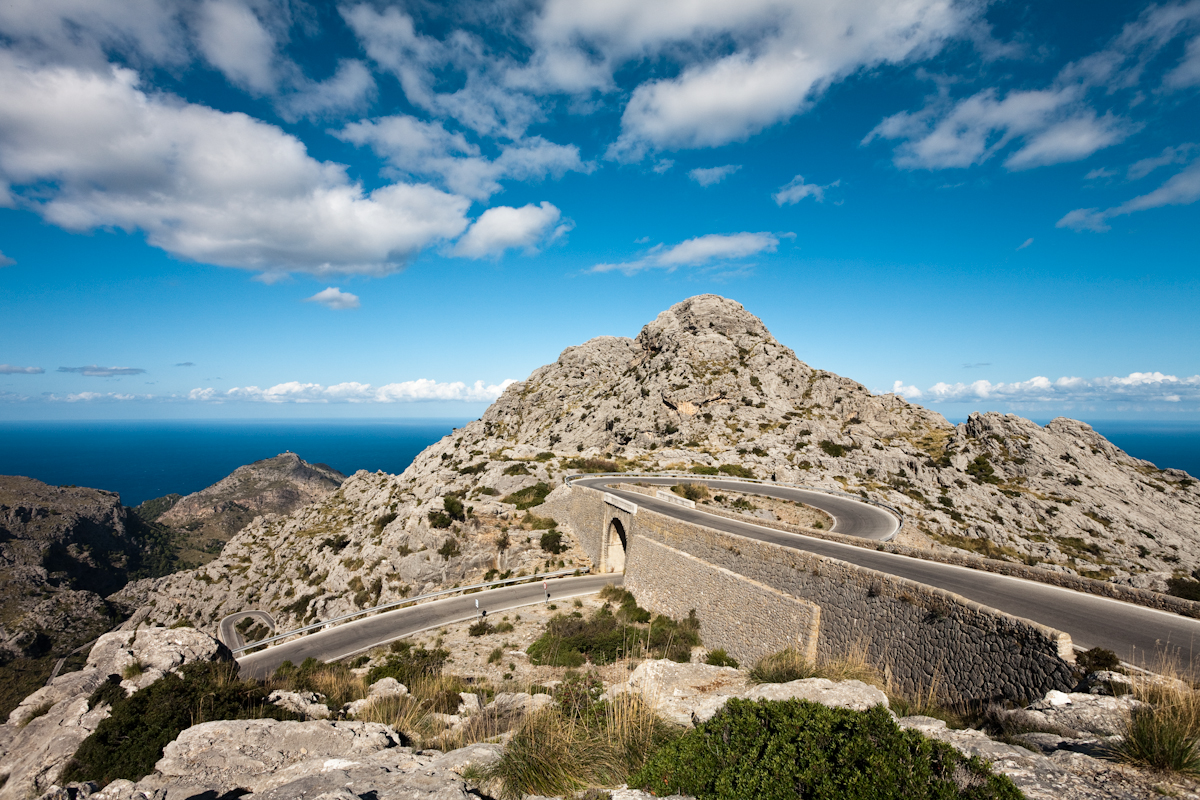
\includegraphics[width=\textwidth]{content/00_LaTeX/exampleProject/images/b1.jpg}
		\subcaption{Subfigure Bild Nr. 1}
	\end{subfigure}
	\begin{subfigure}[c]{0.49\textwidth}
		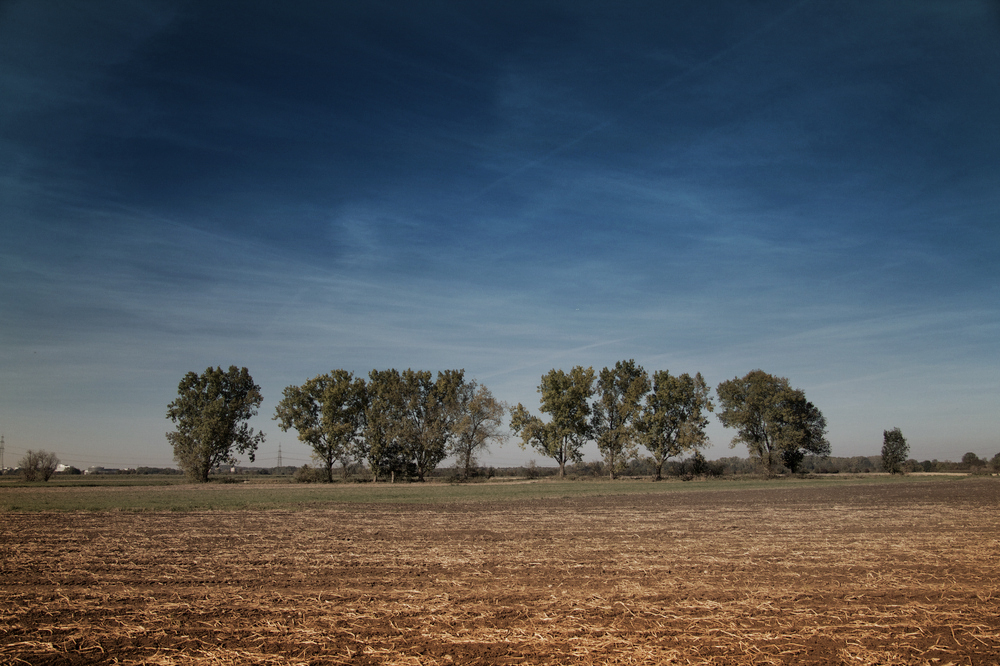
\includegraphics[width=\textwidth]{content/00_LaTeX/exampleProject/images/b2.jpg}
		\subcaption{Subfigure Bild Nr. 2}
	\end{subfigure}
	\caption{Zwei Bilder mit Subfigure nebeneinander}
\end{figure}

Dagegen gibt es die \texttt{wrapfigure} Umgebung, die das Einbinden von Grafiken im Fließtext erlaubt.
Diese Umgebung ist allerdings ab und zu problematisch zu benutzen.
Tipp: Die \texttt{wrapfigure} Umgebung vor dem Absatz platzieren und darauf achten, dass sie nicht in der Nähe eines Seitenumbruchs ist.
Dann erscheint sie rechts oder links des Paragraphen. Mit \texttt{vspace} kann noch der Abstand nach oben und unten angepasst werden, um leeren Platz zu vermeiden.
Siehe auch \url{https://tex.stackexchange.com/questions/56176/handling-of-wrapfig-pictures-in-latex}.

\begin{figure}[ht]
	\centering
	
\includegraphics[width=0.50\textwidth]{content/00_LaTeX/exampleProject/images/desktop-screen.pdf} 
	\caption{Desktop Ansicht mit einem Symbol}
	\label{fig:Referenz-auf-Bild}
\end{figure}

Das kostenlose Tool \href{https://inkscape.org/}{\textbf{Inkscape}} hilft dir beim erzeugen dieser SVG Grafiken. Solltest du noch nie damit gearbeitet haben, dann schau dir am besten einige kurze Tutorials an. Im Github Repository unter dem Reiter Wiki findest du eine Kurzanleitung, wie du ein PDF in Inkscape generieren kannst. Solltest du weitere gute kostenlose Software für die Bildbearbeitung in SVG kennen, dann kannst du diese gerne uns per E-Mail mitteilen. Danke!

\section{Diagramme, Mockups, Software Design}

Um Software Designs mit einzubinden eignet sich das Online Tool \textbf{\href{https://www.draw.io/}{DRAW.IO}} sehr gut. Mit diesem Tool lassen sich Diagramme, Mockups, Flow Charts, technische Zeichnungen, Wireframe Skizzen sowie Software Designs zeichnen, welche du ohne Verpixelung im PDF-Format wieder, wie in Abbildung \ref{fig:Diagramm-DrawIo} gezeigt, einbinden kannst.

\begin{figure}[ht]
	\centering
	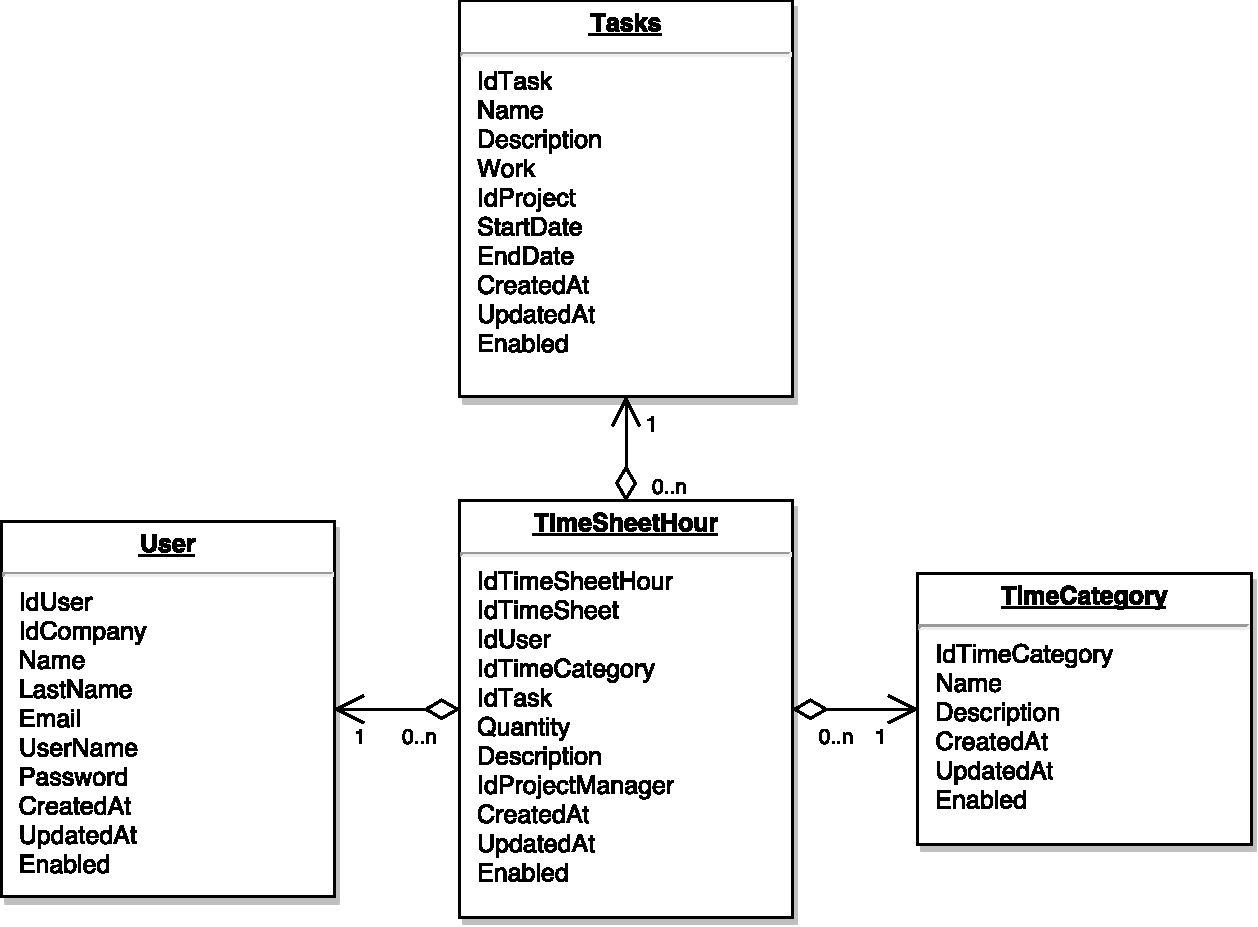
\includegraphics[width=0.8\textwidth]{content/00_LaTeX/exampleProject/images/Diagramm.pdf} 
	\caption{Diagramm eines Software Designs}
	\label{fig:Diagramm-DrawIo}
\end{figure}

Ein weiteres kostenloses Tool für die Darstellung von Klassendiagrammen oder auch Sequenzdiagrammen ist \textbf{\href{http://staruml.io/}{StarUML}}. Dieses generiert auch SVG Dateien, welche du mithilfe von Inkscape zu PDF Dateien konvertieren kannst.

		\chapter{Textformatierungen}

\section{Definitionen und Highlight Boxen}

\begin{defStrich}[Definition]
Diese Hervorhebungen können für deine Arbeit an machen stellen sehr nützlich sein. Besonders bei Definitionen macht es einen guten Eindruck, wenn diese in solch einer Form dargestellt ist. 
\end{defStrich}

DHBW Richtlinie: Laut den aktuellen Angaben der DHBW sind diese Boxen nicht notwendig. Helfen können sie jedoch, um einen Faktor speziell hervorzuheben. Bitte beachte, dass deine Projektarbeit oder auch Bachelorarbeit kein Bilderbuch ist! Alles was eingebunden wird sollte schlicht und dezent dargestellt sein.

\bigskip

\begin{defEckKasten}[Wichtig] Verwende kein \glqq ich\grqq{}, während der gesamten Arbeit. Jeder weiß, dass es deine Arbeit ist. Auch von Sätzen mit \glqq man\grqq{}, solltest du Abstand nehmen. Frage deinen Betreuer gerne, welche Vorzüge er oder sie hat. Jeder Dezi oder DHBW-Betreuer hat in diesem Zusammenhang unterschiedliche Meinungen.
\end{defEckKasten}

\section{Schriftbild}
% Größe
{\LARGE LARGE Text} {\small small Text} normal Text

% Fett, KAPITÄLCHEN, Kursiv
\textbf{Fetter Text} \textsc{Großbuchstaben} \textit{Kursiver Text}

% Schreibmaschinenschrift, serifenlose Schrift, Serifenschrift
\texttt{Schreibmaschinenschrift} \textsf{serifenlose Schrift} \textrm{Serifenschrift}

Manche Zeichen wollen einfach nicht so, wie der Autor das will: \% \& \$ \{ \}

\newpage

\section{Listen}

%Bulletpoints und eigene Symbole
\begin{itemize}
	\item Erster geworden
	\begin{itemize}
		\item Wir sind nicht oben oder?
		\item[+] Nummerierungen oder
		\item[-] Aufzählungen oder
		\item[*] Definitionen 
	\end{itemize}
\end{itemize}

% Nummerierte Liste oder festgelegte Nummer
\begin{enumerate}
	\item Jetzt ist es offiziell ich bin die Nummer 1
	\item[42.] Es ist die Antwort auf alles
\end{enumerate}

\begin{description}
	\item[Epidemie / Pandemie] \hfill \\
	Als Epidemie bezeichnet man eine in einem bestimmten begrenzten Verbreitungsgebiet auftretende ansteckende Erkrankung; eine Seuche, für die typisch ist, dass eine große Zahl von Menschen gleichzeitig befallen wird.
\end{description}


\section{Abkürzungen}
Während du schreibst benötigt du zu manchen Zeitpunkten einfach ein paar Abkürzungen. Doch wie mache ich das wenn ich eine Abkürzung für die \acp{API} nutzen möchte. Ich könnte auch nur ein \ac{API} gemeint haben. Daneben gibt es noch \ac{HTTPS} oder \ac{AJAX}. Willst du einen Begriff nochmals ausschreiben, dann verwende \acf{HTTPS} einfach als Kommando.

Du kannst auch den Plural von Abkürzungen verwenden. Dazu einfach ein \texttt{p} an den jeweiligen Befehl anhängen, z.B. 
\acfp{ISBN}.

Im Text können gewisse Dinge auch nützlich sein wie \zB diese Abkürzung, \dash du kannst sie so direkt in den Text eintragen. Die Namen kann jeder selbst festlegen.


\section{Anführungszeichen}

Normale Anführungszeichen (\"{}) können in \LaTeX{} nicht verwendet werden. Dafür muss das entsprechende Wort in \texttt{\textbackslash enquote{\{\ldots\}}} gesetzt werden. Beispiel: \enquote{Ich stehe ich Anführungszeichen. \enquote{Schachtelungen funktionieren auch.}}

Alternativ können Anführungszeichen auch von Hand gesetzt werden:
\texttt{\textbackslash glqq\{\}} entspricht \glqq{} und \texttt{\textbackslash grqq\{\}} entspricht \grqq{}

\section{Verweise und URLs}\label{sec:verweise}
URLs können mit dem Package \enquote{hyperref} und den Befehlen \texttt{href} und \texttt{url} dargestellt werden. Beispiele:

\begin{itemize}
	\item Mit eigenem Text: \href{https://github.wdf.sap.corp/vtgermany/LaTeX-Template-DHBW/}{\textbf{Klick mich}, um diese Vorlage auf Github zu sehen!}
	\item Anzeigen der URL: \textbf{\url{https://www.google.com/}}
\end{itemize}

Verweise sind eines der wichtigsten Werkzeuge von \LaTeX. Mit dem Package \enquote{hyperref} gibt es verschiedene Verweise, die in \autoref{tabelle:verweise} gelistet sind.

\begin{table}[ht]
	\centering
	\begin{tabular}{rll}
		        \texttt{\textbackslash ref} & Zeigt die Nummer                   & Bsp.: \ref{sec:verweise}                   \\
		    \texttt{\textbackslash autoref} & Zeigt Typ + Nr.                    & Bsp.: \autoref{sec:verweise}               \\
		\texttt{\textbackslash autopageref} & Zeigt \enquote{Seite Seitennummer} & Bsp.: \autopageref{sec:verweise}           \\
		    \texttt{\textbackslash nameref} & Zeigt den Namen (bzw. Caption)     & Bsp.: \nameref{sec:verweise}               \\
		   \texttt{\textbackslash hyperref} & Eigener Text                       & Bsp.: \hyperref[sec:verweise]{Klick mich!}
	\end{tabular}
	\caption{Verweise im Dokument}
	\label{tabelle:verweise}
\end{table}

		% LTeX: enabled=false
\chapter{Mathematik}

\section{Text}
Hier steht ein beispielhafter Text bei dem nun auf eine sehr bekannte und durchaus vertraute Formel im Text direkt mit $c = \sqrt{a^2 + b^2}$ eingegangen wird. Dabei können auch Winkel wie: $\alpha, \beta, \gamma$ gerne verwendet werden. Weiterhin werden hier nur Formeln im Bereich der $\mathbb{N}$ dargestellt, gerne können diese aber durch Formeln aus diesem Bereich der $\mathbb{R}$ ergänzt werden.

\section{Formeln}
Beachte bei Formeln keine konkreten Werte anzugeben, sondern die Formel stets nur wie in der Literatur nur als Größengleichungen anzugeben.
\begin{align}
	\sum_{n=0}^{\infty}x=b+n\\
	\frac{b*x}{c} = y
\end{align}

Trotz unterschiedlicher Länge kann man die Gleichheitszeichen auf der gleichen Höhe anbringen wie in \autoref{eq:Gleichung1} und \autoref{eq:Gleichung2} dargestellt, zusätzlich kann man diese auch mit Informationen versehen wie in Formel \autoref{eq:Gleichung3} zu sehen.

\begin{align}
	\label{eq:Gleichung1} a + b &= c\\
	\label{eq:Gleichung2} 5c + 3f &= 4h\\ 
	\label{eq:Gleichung3} \overbrace{5y}^{y = 0} + \underbrace{42x}_{x = 1} &= b
\end{align}

\section{Arrays und Matrizen}

\begin{center}
	\(
	\begin{array}{lc|r}
		a&b&c\\
		\hline
		x&y&z\\
		c&a&b
	\end{array}
	\)
\end{center}

\begin{equation}
	\begin{array}{lcl}
		z & = & a \\
		a + b & = & c \\
		f(x,y,z) & = & x + y + z
	\end{array}
\end{equation}

Hier noch ein paar Matrizen Beispiele in \LaTeX{}.

\begin{align}
	\begin{pmatrix}
		a_{11}	& \dots   & a_{1n}\\
		\vdots	& \ddots  & \vdots\\
		a_{n1}	& \dots   & a_{nn}\\
	\end{pmatrix}
	\\[0.4cm]
	\begin{bmatrix} 
		100&250\\
		300&499
	\end{bmatrix}
	\\[0.4cm]
	\begin{Bmatrix} 
		100&250\\
		300&499
	\end{Bmatrix}
	\\[0.4cm]
	\begin{Vmatrix}
		100&250\\
		300&499
	\end{Vmatrix}
\end{align}

\section{Klammern und Kästchen}

\begin{center}
	\( \Vert x\Vert_{p}=
	\left(
	\sum_{i=1}^{n} | x_{i} |^{p}
	\right)^{\frac{1}{p}} \)
\end{center}

\begin{center}
	\( \left.
	\begin{array}{lc|r}
		a&b&c\\
		\hline
		x&y&z\\
		c&a&b
	\end{array}
	\right\}
	\Rightarrow z,b \)
\end{center}

\begin{equation*}
\mbox{
	\boxed{
		\sin^2\varphi+\cos^2\varphi=1
	}
}
\end{equation*}


Eine beispielhafte Formelabkürzung: 
\ac{A}

		% LTeX: enabled=false
\chapter{Programm- bzw. Quellcode}
\section{Quellcode}
Ein wichtiger Punkt ist auch, dass man Quellcode Stücke mit in seinen Praxisbericht einbaut. Hier nun einfach mal ein Beispiel in Form eines kleinen JAVA Codes, welcher aus einer Datei gelesen wird:

\lstinputlisting[
	label=code:algQuersumme,    % Label; genutzt für Referenzen auf dieses Code-Beispiel
	caption=Algorithmus zur Berechnung der Quersumme,
	captionpos=b,               % Position, an der die Caption angezeigt wird t(op) oder b(ottom)
	style=EigenerJavaStyle,     % Eigener Style der vor dem Dokument festgelegt wurde
	firstline=3,                % Zeilennummer im Dokument welche als erste angezeigt wird
	lastline=18                 % Letzte Zeile welche ins LaTeX Dokument übernommen wird
]{sourceCode/Eigenes-Java-File.java}

Zu beachten ist, dass jedes Stück Code kommentiert werden sollte. Was wird in diesem Abschnitt genau durchgeführt. Wo könnten Probleme auftreten und warum wurde dieses Stück hier hinzugefügt.

\vspace*{0.5cm}

\pagebreak

Es ist auch möglich, innerhalb des Listings \LaTeX{} Befehle zu verwenden. Dazu muss aber eine Escape-Sequenz angegeben werden. Das folgende Beispiel enthält ein Label, auf das dann verwiesen werden wird: Auch hier funktioniert \texttt{\textbackslash{}autoref}: \enquote{In \autoref{code:var_b} wird der Variable \texttt{b} \ldots}.

\begin{lstlisting}[
  style=EigenerJavaStyle,
  captionpos=b,
  caption={Zuweisung von Variablen},
  label={code:basic_block},
  escapeinside={@}{@}]
int a = 10;
@\label{code:var_b}@int b = a + 20;
return;
\end{lstlisting}

\pagebreak
Weitere Programmiersprachen können auch eingebunden werden. Hier mal ein Beispiel in der Programmiersprache Python:
\lstinputlisting[
	label=code:WhileLoop,    % Label; genutzt für Referenzen auf dieses Code-Beispiel
	caption=Algorithmus zum schätzen einer Zahl in Python,
	captionpos=b,               % Position, an der die Caption angezeigt wird t(op) oder b(ottom)
	style=EigenerPythonStyle,   % Eigener Style der vor dem Dokument festgelegt wurde
	firstline=0,                % Zeilennummer im Dokument welche als erste angezeigt wird
	lastline=23                 % Letzte Zeile welche ins LaTeX Dokument übernommen wird
]{sourceCode/Eigenes-Python-File.py}

\clearpage % Absichtlicher Seitenumbruch, um ein besseres Layout zu erhalten.

\section{Pseudocode}
Pseudocode kann hilfreich sein, wenn \enquote{richtig} implementierte Algorithm in einer Programmiersprache zu lang sind und diese mittels Pseudocode bündig zusammengefasst werden können. \autoref{lst:euclid} zeigt Pseudocode.

Die Doku für das Package und damit eine Liste aller Befehle findet sich 
\href{http://tug.ctan.org/macros/latex/contrib/algorithmicx/algorithmicx.pdf}{hier}

\begin{algorithm}
	\caption{Euclid's algorithm}\label{lst:euclid}
	\begin{algorithmic}[1]
		\Procedure{Euclid}{$a,b$}\Comment{The g.c.d. of a and b}
			\State $r\gets a\bmod b$
			\While{$r\not=0$}\Comment{We have the answer if r is 0}
				\State $a\gets b$
				\State $b\gets r$
				\State $r\gets a\bmod b$
			\EndWhile\label{euclidendwhile}
			\State \textbf{return} $b$\Comment{The gcd is b}
		\EndProcedure
	\end{algorithmic}
\end{algorithm}
		\chapter{Literaturhinweise}

\textbf{Hinweis}: Verwendest du eine Quelle nicht, dann nimmt \LaTeX{} diese nicht mit ins Literaturverzeichnis auf!

\section{Fußnoten und Literaturverweise}
Hamburger, Döner, Currywurst\footnote{Hier fehlt eindeutig das Lieblingsessen der Informatiker, die Pizza!} - jeder kennt sie, jeder liebt sie und jeder isst sie.
Weil die Zeit drängt\cite{ahk:001}, der Hunger groß ist und der nächste Schnellimbiss\cite{bpb:001} nur drei Schritte voraus. Und nach dem Essen?
Sind wir zwar satt, aber meist nicht wirklich glücklich, weil Fastfood\cite{bpb:006} meist eben auch nicht wirklich gut ist \cite{bpb:005}.

Ja, uns ist bewusst, dass die Literatur nicht zum Text passt.
Deswegen hier nochmals der Rest.\cite{eur:001,EU:001,Lang1998,höl:001,wdb:001}

Übrigens: \acfp{ISBN} gehören nicht in die Bibliographie und werden deshalb auch nicht angezeigt.

	}
	
	% -- Einbinden des Literaturverzeichnisses 
	\cleardoublepage												% Beendet eine Seite
	\renewcommand*{\chapterpagestyle}{plain}						% Kapitel-Style wird auf plain gestellt 
	\pagestyle{plain}												% Seiten-Style wird auf plain gestellt			
	\pagenumbering{Roman}                   						% Römische Seitenzahlen
	\setcounter{page}{\numexpr\value{savepage}+1}					% Zähler der römischen Zahlen wird inkrementiert
	\printbibliography[title=Literaturverzeichnis]					% Literaturverzeichnis wird erstellt
	
	% -- Einbinden des Glossars
	\printglossary[style=altlist,title=Glossar]						% Glossar wird erstellt

    % -- Einbinden von Anhängen
    \begin{appendices}
		\renewcommand{\indexname}{Stichwortverzeichnis}
\printindex

	\ifthenelse{\boolean{abgabeVersion}}
	{}
	{
		\chapter{Uninteressanter Anhang}
Dies Anhang besitzt eigentlich keinen Sinn, außer einen Platzhalter im Inhaltsverzeichnis zu erzeugen.
	} 	
    \end{appendices}
\end{document}